\documentclass[a4paper, 11pt]{report}

\usepackage{hyperref}
\usepackage[left=4cm,right=4cm,top=4cm,bottom=4cm]{geometry}
\usepackage[french]{babel}
\usepackage[utf8]{inputenc}
\usepackage[OT1]{fontenc}
\usepackage[export]{adjustbox}
\usepackage[standard]{ntheorem}
\usepackage{array,multirow,makecell}
\usepackage{graphicx}
\usepackage{pdftricks}
\usepackage{listings}
\usepackage{color}
\usepackage{impnattypo}
\usepackage{acronym}
\usepackage[section]{placeins}
\usepackage{pdfpages}
\usepackage{lmodern}
\usepackage{titling}

\begin{document}

\graphicspath{ {images/} }

\title{{
\includegraphics[width = 50mm]{./logos/logo-epsi-v2.png}}{
\includegraphics[width = 50mm]{./logos/logo-quartz-insight-v2.png}}\\[2cm]Dossier Professionnel: Expert / Experte en informatique \& Système d’Information (EISI)}
\author{Brunet Geoffrey}
\date{Année scolaire 2022/2023}
\renewcommand{\maketitlehookb}{\centering Entreprise: Quartz Insight, École: EPSI campus d'Auxerre}
\maketitle

\definecolor{dkgreen}{rgb}{0,0.6,0}
\definecolor{gray}{rgb}{0.5,0.5,0.5}
\definecolor{mauve}{rgb}{0.58,0,0.82}

\lstset{frame=tb,
    language=Java,
    aboveskip=3mm,
    belowskip=3mm,
    showstringspaces=false,
    columns=flexible,
    basicstyle={\small\ttfamily},
    numbers=none,
    numberstyle=\tiny\color{gray},
    keywordstyle=\color{blue},
    commentstyle=\color{dkgreen},
    stringstyle=\color{mauve},
    breaklines=true,
    breakatwhitespace=true,
    tabsize=3
}

\tableofcontents

\chapter{Remerciements}
Je tiens à exprimer mes plus sincères remerciements à l’entreprise Quartz Insight, notamment à M. Christian MONTILLAUD, gérant et fondateur de l’entreprise pour m'avoir accueilli au sein de sa société ainsi qu'à M. Gaël ROUSTAN, Chief Technical Officer et tuteur pour m'avoir encadré tout au long de ma formation.
Je tiens à remercier également tous les collaborateurs du pôle "recherche et développement" qui comme mon tuteur ont pris le temps de m’apporter leur aide sur les projets qui me sont confiés, ce qui m’a permis de monter en compétences tout au long de l’année.
\newline
\newline
Mes remerciements vont aussi vers les membres du personnel de l’EPSI Auxerre pour leur confiance et les formations prodiguées.
L’enseignement de qualité du titre professionnel « Expert en Informatique et système  d’information »  a parfaitement été en adéquation avec mes objectifs tout au long de l’année. 
Plus spécifiquement, je tiens à remercier monsieur Sébastien Guilbert (responsable Business Unit Enseignement supérieur au pôle formation 58-89) pour sa confiance pour mon intégration au sein de l’EPSI, et ayant apporté son aide autant sur des plans professionnels que personnels.
\newline
\newline
J’aimerais aussi exprimer ma gratitude envers tous les formateurs étant intervenus tout au long de cette année de bachelor, qui ont pris le temps de nous préparer et de fournir des formations de qualité, et écouter nos difficultés lorsque nous en avions.
\newline
\newline
Pour finir, je tiens à présenter ma gratitude et mon respect à toutes les personnes qui m'ont accompagné tout au long de mon parcours pour le temps qu'ils m'ont consacré dans le but de faire de moi un meilleure développeur.

\chapter{Introduction}

Quartz-Insight est une société créée en 2015 par monsieur Christian Montillaud suite à une volonté de fonder une entreprise basée sur l’expertise,  la performance et le management des processus d’EPM et de BI des entreprises.
L’origine du nom de l’entreprise proviens de la passion de monsieur  Montillaud pour les minéraux, et le Quartz étant choisis car étant un minéral transparent, valeur qu’il souhaite apporter à son entreprise.
Le terme «Insight » quand à lui reprend la volonté d’avoir une expertise profonde, une véritable introspection sur les domaines de compétences de l’entreprise.
\newline
\newline
Les trois valeurs de l’entreprise sont l’accompagnement (de l’écoute à la proposition d’une solution adaptée), l’esprit d’équipe (allant de paire avec la solidarité) et l’honnêteté (avec nos différents clients et parternaires).
\newline
\newline
Ses activités sont principalement basé sur les solutions logicielles EPM  de chez Oracle, allant d’outils comme Essbase, une base de données multidimensionnelle à Planning, ne solution de planification et de budgétisation.
Quart-Insight a deux pôles d’activités différents.
Le premier est un pôle « consulting », les collaborateurs membres apportant leurs expertises aux clients pour la gestion et l’amélioration de leurs différents services EPM.
Le deuxième pôle est un pôle Recherche et Développement, avec une équipe d’ingénerie travaillant sur une solution logicielle sous forme d’Add-In pour la manipulation de logiciels de BI dans des tableurs ou logiciels de présentation comme Microsoft Excel, Google Sheets et Google Slides.    
\clearpage

\chapter{Environnement professionnel}
\section{Organigramme de Quartz-Insight}
\begin{figure}[h]
    \centering
    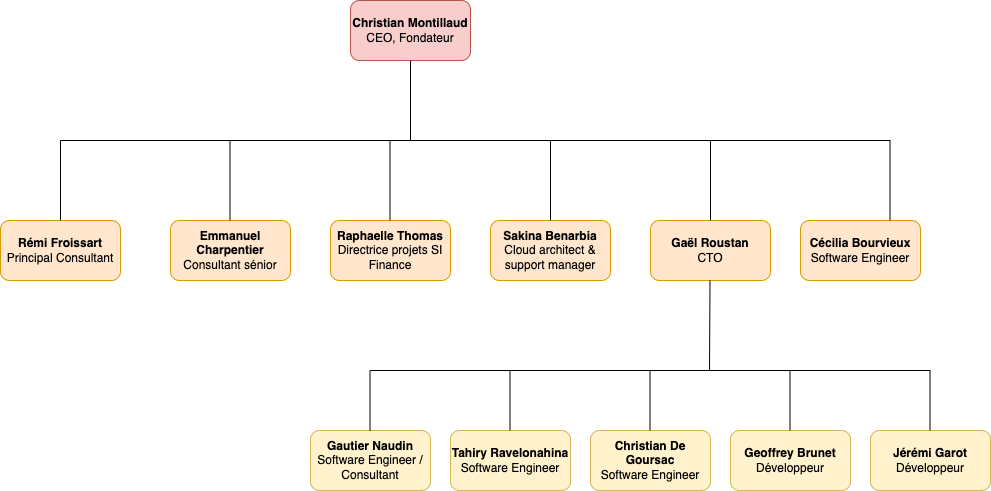
\includegraphics[scale=0.50,center]{schemas/organigramme-quartz-insight.png}
    \caption{Organigramme de Quartz-Insight}
\end{figure}
La société est gérée par monsieur Christian Montilaud.
Monsieur Gaël Roustan, est directeur technique et supervise le pôle Recherche et Développe\-ment.
Madame Cécilia Bourvieux gère un projet de test de charge pour les solutions de BI, du développement logiciel à la mise en place et l’exécution chez les clients.
Les membres du pôle R\&D ont en charge le développement des Add-Ins pour les logiciels de chez Microsoft et Google, ainsi que la création, la mise en production et la gestion des microservices sous-jacents, avec l’aide de notre CTO.
Le reste des collaborateurs sont des consultants apportant leurs expertises dans leurs domaines respectifs chez nos différents clients.
\newline
\newline
Je suis donc actuellement développeur au sein du pôle R\&D, et travaille sur différents projets et microservices, dans le but d’améliorer ceux existants, résoudre des bugs et en créer de nouveaux lorsque cela est nécessaire.

\begin{figure}
  \section{Présentation de l'étudiant}
  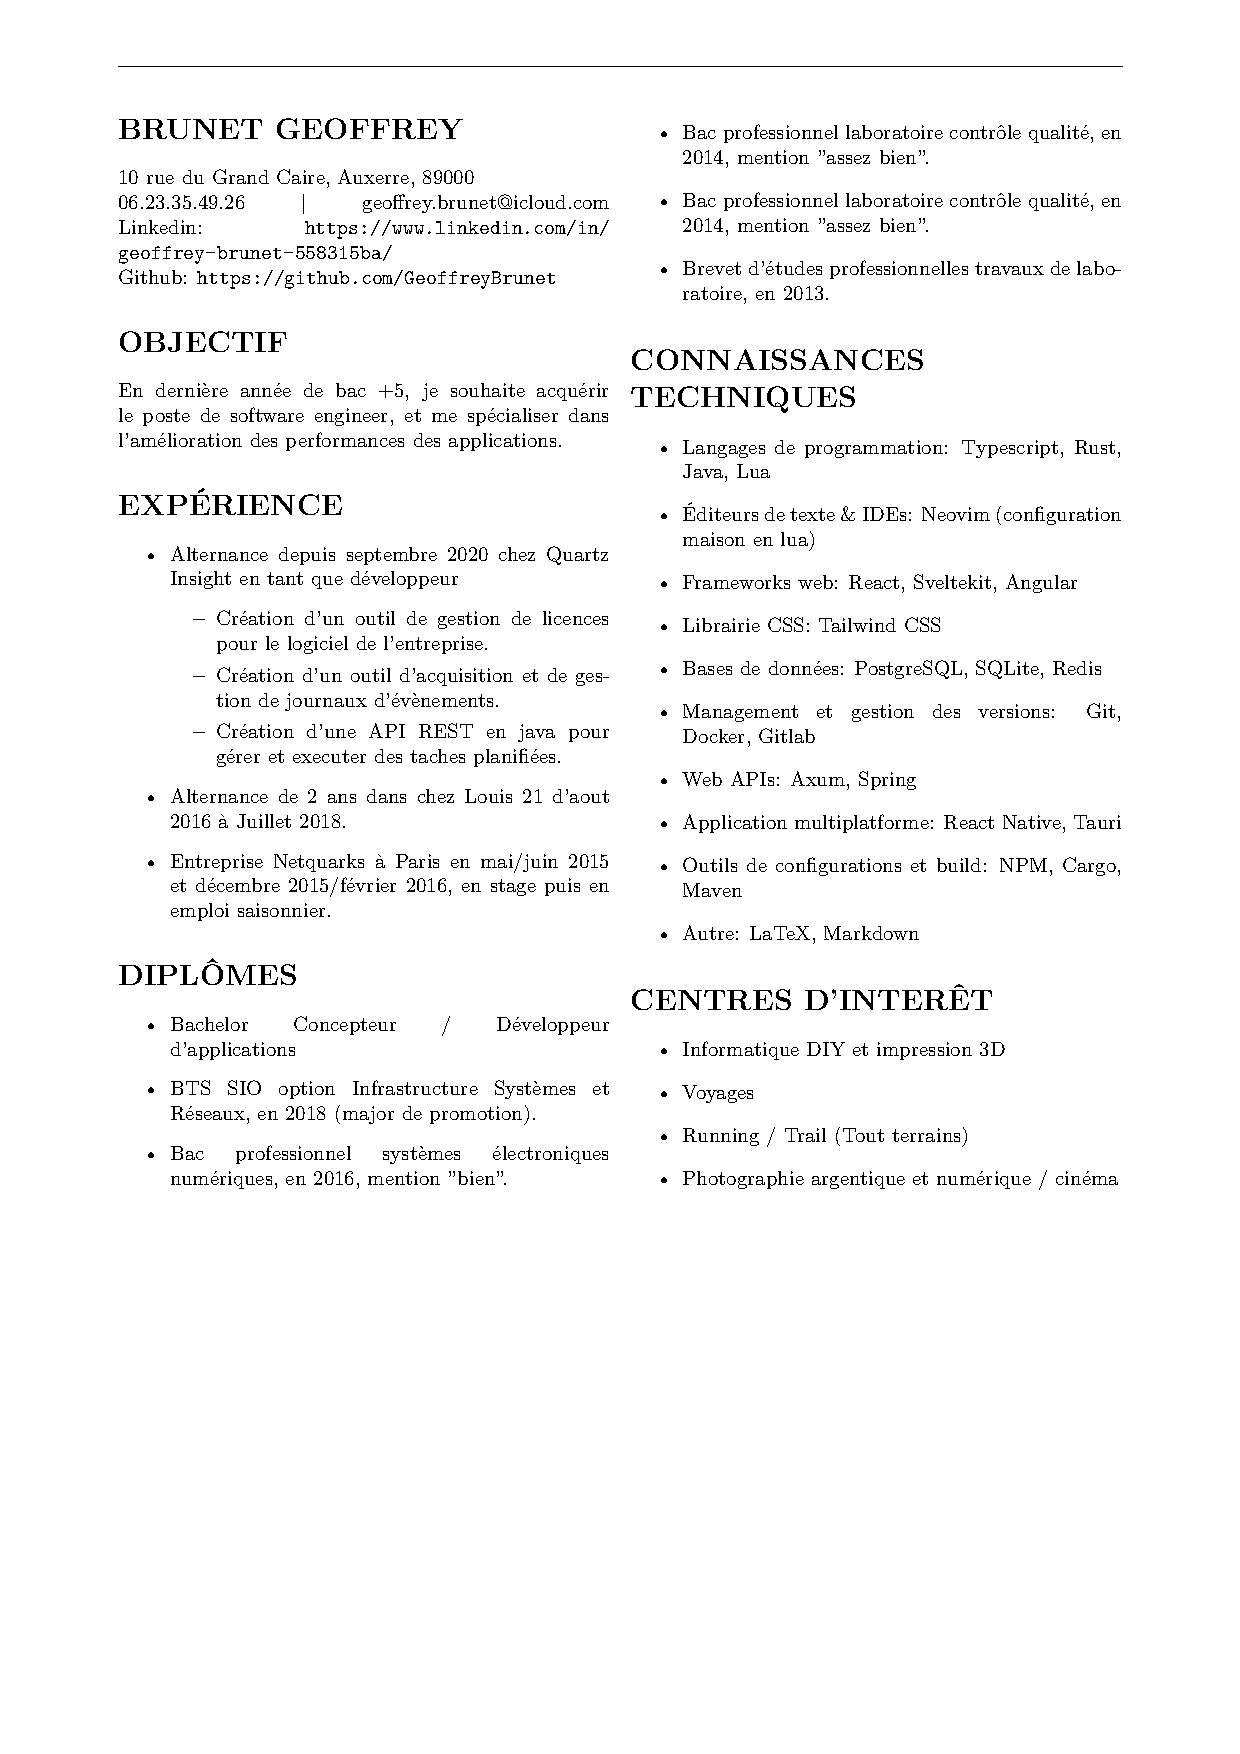
\includegraphics[scale=0.85, trim=2cm 0 0 0, clip]{CV-Geoffrey-Brunet.pdf}%
\end{figure}

\section{Activités de la structure}
Quartz-Insight est une entreprise spécialisée dans la Business Intelligence (BI) et l'Enterprise Performance Management (EPM).
Elle propose une gamme complète d'activités et de services destinés à aider les entreprises à optimiser leur gestion et à prendre des décisions éclairées. Voici un aperçu de nos principales activités:
\begin{enumerate}
  \item \textbf{Consulting en BI et EPM}: Quartz-Insight offre des services de consulting personnalisés pour accompagner les entreprises dans leur utilisation efficace des outils de BI et d'EPM tels que les serveurs Essbase, les cubes OLAP et Hyperion Planning.
    \ Les consultants de Quartz-Insight travaillent en étroite collaboration avec les clients pour comprendre leurs besoins spécifiques et proposer des solutions adaptées à leurs objectifs.
  \item \textbf{Réalisation de tests de charges sur des infrastructures de BI et d’EPM}: nous proposons une prestation de tests de charges pour les infrastructures BI et EPM des entreprises, avec divers scénarios possibles, pour tester les limites du matériel physique comme du logiciel.
    \ Le produit final est un fichier PDF contenant les résultats sous forme de graphs, ainsi qu’une proposition d’actions à mettre en place pour améliorer la résilience de l’infrastructure.
  \item \textbf{Développement de Qibates}: développement d’un logiciel en mode SAAS (Software As A Service) pour explorer diverses sources de bases de données multidimensionnelles.
    \ Un abonnement par licence par utilisateur est proposé à la vente, pour une utilisation sur Microsoft Excel ou Google Sheets, avec des accès à des sources de données diverse grâce à des connecteurs développés par nos soins. 
  \item \textbf{Conseil sur la transition RSE des entreprises}: après une implementation d’actions RSE (Responsabilité sociétale des entreprises) et de formations pour notre entreprise, nous avons décidé de proposer à nos clients une formation comprenant tous les principaux axes des actions mises en place.
    \ Nos proposons aussi une animation pour la fresque du climat, pour démontrer l’implication écologique pour les personnes comme pour les entreprises.
\end{enumerate}

\section{Présentation des activités confiées}
Voici une liste contenant les tâches qui m’ont été confiées durant mon alternance chez Quartz-Insight:
\begin{itemize}
  \item Écriture de fichiers « Dockerfile » pour la conteneurisation de nos microservices
  \item Résolution de tickets d’incidents sur l’add-in QiBates pour Google Sheets
  \item Écriture d’un logiciel de récupération de journaux d’évènements, avec une page web pour les consulter
  \item Collaboration pour développer une API REST sur un projet pour un de nos client (BNP)
  \item Transformation d’un ancien service monolithique en microservices pour la gestion des licences utilisateurs
\end{itemize}

\section{Présentation du Système d’Information}
Comme vu précédemment, le pôle Recherche et Développement édite des logiciels sous forme d’Add-In pour Google Sheets, Google Slides et Microsoft Excel, pour la manipulation de bases de données multidimensionnelles et d’outils de Planning.
Pour un soucis de performance, le traitement des données n’est pas fait sur le frontend de nos Add-Ins mais par des microservices hébergés sur nos machines virtuelles, dans un format de conteneur Docker.
\newline
\newline
Tous les microservices nécessitant d’être déployé sur des serveurs le seront sur des machines virtuelles hébergées chez notre partenaire OBS (pour Orange Business Services, filiale cloud du groupe Orange).
Ces machines virtuelles utilisent Docker pour gérer les cycles de vie des conteneurs.
Il en vas de même pour les bases de données, que nous utilisons en version managée, donc dont toute la partie serveur est gérée par OBS directement.

\chapter{Valorisation des compétences}

\section{Présentation globale du projet}
En tant qu'alternant, le projet qui m'a été confié consistait à effectuer une transformation majeure d'un service existant, passant d'une architecture monolithique à une architecture de microservices.
Le service initial comprenait une web UI, une API REST et une base de données destinées à stocker les informations des utilisateurs, telles que leurs noms, domaines d'entreprise et types de profil.
L'architecture monolithique, qui reposait sur ASP.NET avec SQL Server comme SGBD, présentait des limitations en termes de flexibilité et d'évolutivité.
L'objectif principal était donc de repenser cette infrastructure afin de permettre une évolutivité améliorée et des performances optimisées.
Pour atteindre cet objectif, nous avons adopté une approche basée sur les microservices.
Cela impliquait de diviser le service en plusieurs composants indépendants, chacun étant responsable d'une fonction spécifique.
Ainsi, nous avons pu obtenir une architecture plus flexible, où chaque microservice peut être géré et déployé de manière autonome.
Dans le cadre de cette transformation, nous avons choisi d'utiliser Angular pour la web UI, offrant ainsi une expérience utilisateur réactive et enrichissante.
Pour l'API REST, nous avons opté pour Spring Boot, un framework Java réputé pour sa simplicité et sa robustesse.
De plus, nous avons migré la base de données vers PostgreSQL, un système de gestion de base de données open source réputé pour ses performances et sa fiabilité.
Toutes ces technologies sont identiques pour le reste de nos microservices, nous permettant d’avoir une architecture uniformisée.

\section{Activité 1 - cartographie complète du système d'information existant}
\subsection{Compétence et son fondement}
\textbf{Bloc de compétences}: A1 – Analyse et définition de la stratégie des systèmes d’information
\newline
\textbf{Compétence choisie}: A1C4 – Cartographier un système d’information existant selon les 4 niveaux (métier, fonctionnel, applicatif et infrastructure) afin d’avoir une bonne connaissance de l’ensemble de ses composants
\newline
\textbf{Détails}: Cette compétence consiste à valider mon aptitude à réaliser une cartographie du S.I. précisant pour chaque couche les éléments suivants:
\begin{itemize}
  \item préciser dans le schéma les entités et les systèmes (en lien avec les Process Métier)
  \item préciser l’architecture applicative globale (les logiciels, les services et l’analyse des flux de données)
  \item présenter dans son schéma l’Infrastructure logique (VLAN, adresse.IP, filtrage et routage) infrastructure physique (équipements).
\end{itemize}
Elle consiste aussi à démontrer une utilisation appropriée d’un logiciel de cartographie:
\begin{itemize}
  \item démarrage du logiciel adéquat
  \item temps d’utilisation approprié (min 10 minutes)
  \item le résultat de la cartographie informatique correspond aux attendus d’une cartographie d’un SI demandé par un comité de direction
\end{itemize}
\subsection{Présentation et réalisation de l'activité}
Une étape pour cartographier le système d'information existant selon les 4 niveaux (métier, fonctionnel, applicatif et infrastructure) serait la réalisation d'une analyse approfondie de l'environnement existant. Voici la suite d’étapes réalisées pour atteindre cet objectif:
\subsubsection{Collecte des informations}
Ce monolithe n’a pas de documentation proprement associée, la principale source de connaissance est son code source, présent dans son repository sur Gitlab.
Pour analyser le service monolithique et étant programmé en .net, j’ai utilisé l’IDE fournis par Microsoft, Visual Studio.
Les informations importantes à regarder pendant l’analyse du code sont:
\begin{enumerate}
  \item Les endpoints de l’API REST
  \item Les classes qui servent de modèles
  \item Les requêtes effectuées par l’ORM vers le SGBD
  \item Les autres microservices qui communiquent avec le monolithe.
\end{enumerate}
La base de donnée utilisée par le monolithe a été utile pour observer les données sauvegardées dans les tables, et les jointures entre elles.
Étant donné qu’il s’agit de Microsoft SQL Server comme service de gestion de base de données, j’ai utilisé SSMS (SQL Server Management Studio) pour effectuer mes recherches.
Pour ce qui est des diagrammes et schémas, je les ai réalisé après analyse et sont présent dans ce dossier dans la sous-section « Analyse applicative ».
\subsubsection{Identification des composants métier}
Après consultation de l’équipe de développement, ce service monolithique n’est utilisé que par les dit-membres de cette équipe. La console n’est accéssible et utilisée que par eux.
L’objectif de ce service est de sauvegarder l’état des comptes et domaines clients qui utilisent la solution QiBates, ainsi que le type de profil pour les comptes (qui défini quelles options sont accessibles ou non).
Côté client, si il n’a jamais souscrit à une ou plusieurs licences QiBates, un domaine avec le nom de l’entreprise est créé. Le client envoie une liste des utilisateurs, avec entre autre leurs adresses mails professionnelles, et le type de profile demandé pour chaque compte.
Toutes ces informations sont enregistrées dans un fichier CSV qui est envoyé au monolithe, que celui-ci utiliseras pour créer et écrire les comptes avec les bonnes informations dans la base de données.
\subsubsection{Analyse fonctionnelle}
Pour l'analyse fonctionnelle, j'ai divisé celle-ci en 6 sous-analyses distinctes:
\begin{enumerate}
  \item \textbf{Identification des fonctionnalités, qui sont}:
    \begin{itemize}
      \item Création de profils utilisateur avec des informations telles que leur nom, domaine d'entreprise et type de profil, ainsi que sa durée de validité.
      \item Recherche d'utilisateurs par domaine d'entreprise.
      \item Mise à jour des informations du profil utilisateur.
      \item Gestion de la durée de vie des profils avec possibilité de renouvellement ultérieur.
      \item Suppresion d'un utilisateur, voir d'un domaine.
    \end{itemize}
  \item \textbf{Définition des cas d'utilisation}:
    \begin{itemize}
      \item Demande de création d'un nouvel utilisateur ou de plusieurs utilisateurs par un membre du pôle R&D, avec validation du directeur technique ou du CEO, demande effecutée par un directeur technique ou un contrôleur de gestion, en fonction de nos clients.
      \item Modification d'un profil utilisateur par un membre du pôle R&D, avec validation du directeur technique ou du CEO.
      \item Suppression d'un profil utilisateur par un membre du pôle R&D, avec validation du directeur technique ou du CEO.
      \item Renouvellement de la durée de vie d'un profil utilisateur.
      \end{itemize}
    \item \textbf{Modélisation des flux de travail}:
    Imaginons un premier cas d'utilisation qui serait "Demande de création, modification ou suppression d'un profil utilisateur":
    \begin{itemize}
      \item Un de nos client nous envoie une demande de création, modification ou suppression d'un profil utilisateur avec les informations nécessaires.
      \item Le CEO ou le CTO valide la dite demande.
      \item Les modifications sont transmises au pôle R&D, et un membre de celui-ci apporte les modifications sur l'interface web de l'application.
    \end{itemize}
    Dans le cadre d'un renouvellement de la durée de vie d'un profil utilisateur qui serviras en second cas d'utilisation:
    \begin{itemize}
      \item Un de nos client nous envoie une demande de création, modification ou suppression d'un profil utilisateur avec les informations nécessaires.
      \item Le CEO ou le CTO valide la dite demande.
      \item Les modifications sont transmises au pôle R&D, et un membre de celui-ci apporte les modifications sur l'interface web de l'application.
    \end{itemize}
  \item \textbf{Définition des entrées et sorties}:
    \begin{itemize}
      \item Pour les demandes de création, modification ou suppression d'un profil utilisateur, les entrées comprennent les informations nécessaires pour le profil utilisateur concerné.
      \item Pour la demande de renouvellement de la durée de vie d'un profil utilisateur, l'entrée est l'identification du profil utilisateur concerné.
      \item La sortie attendue est la validation ou le refus de la demande par le directeur technique ou le CEO. Si la demande est validée, la sortie finale est la création, modification ou suppresion d'un ou plusieurs comptes.
    \end{itemize}
\end{enumerate}
\subsubsection{Analyse applicative}
  \begin{figure}[h]
    \centering
    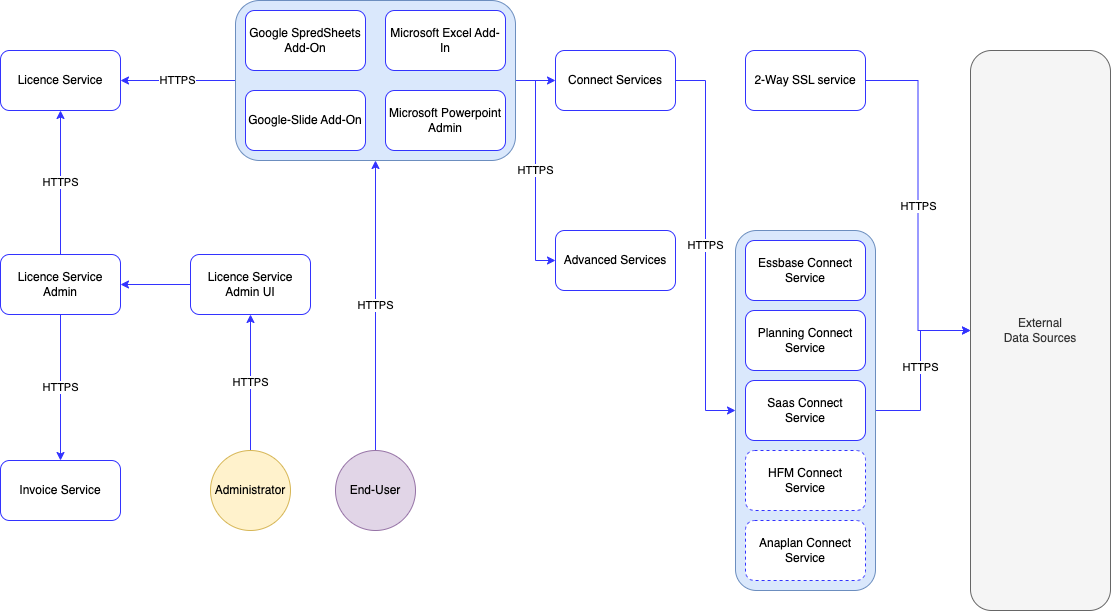
\includegraphics[scale=0.40,center]{schemas/schema-qibates-original.png}
    \caption{Schéma de l'infrastructure actuelle}
  \end{figure}
  Pour plus de clareté et de compréhension des rôles du service monolithique dans le schéma, celui-ci a été fragmenté, mais le monolithe contient tous les services du schéma suivants:
  \begin{itemize}
    \item \textbf{Licence service}: service qui permet de connaître l'existence d'un compte, son état et son profile.
    \item \textbf{Licence service Admin}: Partie backend permettant la création, modification et suppression des comptes, mais uniquement utilisable par un administrateur depuis l'interface web.
    \item \textbf{service Admin UI}: Interface web permettant la création, modification et suppression des comptes.
  \end{itemize}
  \begin{figure}[h]
    \centering
    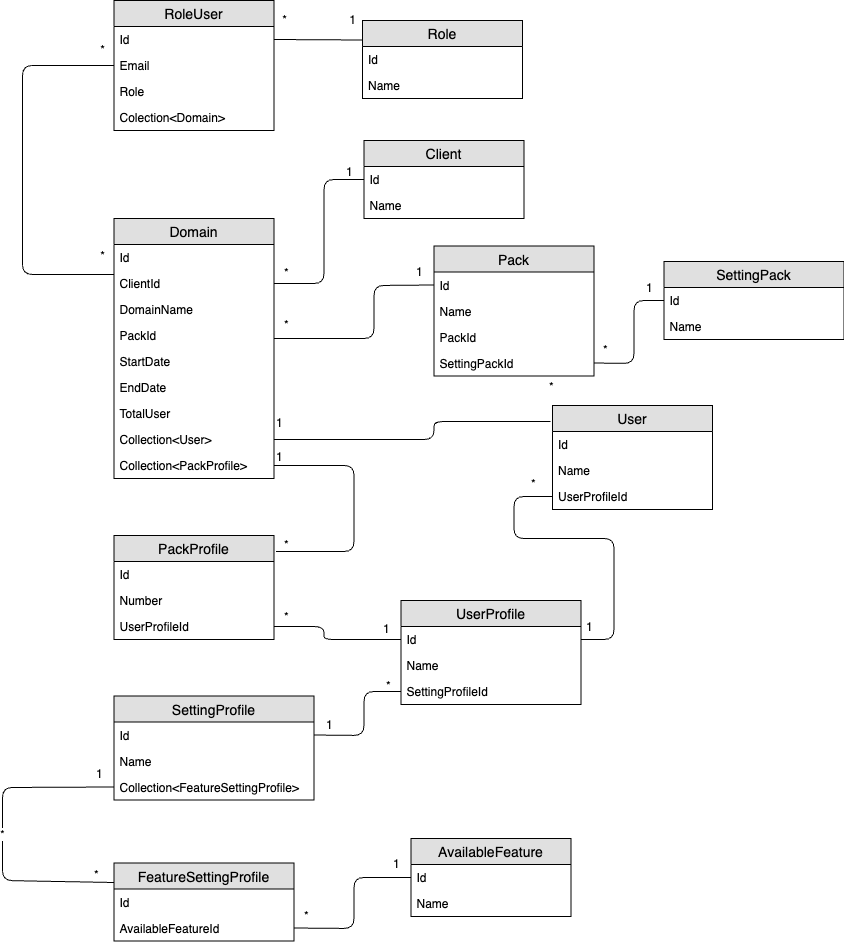
\includegraphics[scale=0.40,center]{schemas/ralph-diagram.png}
    \caption{Modèle de conception de données de la base de donnée du monolithe}
  \end{figure}
  Voici le MCD réalisé à partir des informations obtenues depuis le SGBD, et avec l'aide d'un collaborateur qui avais œuvré à son intégration.
  Une description de l'utilité de chaque table présente dans le schéma est effectuée ici:
  \begin{itemize}
    \item \textbf{Domain}: contient le domaine du client, ainsi que la durée de validité de ses comptes sous-jacents.
    \item \textbf{RoleUser}: utilisateur avec un rôle particulier pour l'administration de l'application.
    \item \textbf{Role}: role d'un utilisateur pour accéder et utiliser la console (droits de lecture ou rôle d'administrateur).
    \item \textbf{Client}: identifiant client, car un client peut avoir plusieurs domaines.
    \item \textbf{Pack}: permet de lier une liste prédéfinie de paramètres à un domaine (pour pouvoir les appliquer à tous les utilisateurs du domaine).
    \item \textbf{SettingPack}: liste prédéfinie de paramètres pour un utilisateur.
    \item \textbf{User}: utilisateur pour utiliser QiBates.
    \item \textbf{PackProfile}: permet de lier un domaine à un utilisateur.
    \item \textbf{UserProfile}: profile utilisateur permettant à un utilisateur d'avoir une liste de paramètres.
    \item \textbf{SettingProfile}: liste de paramètres de fonctionnalitées pour un utilisateurs.
    \item \textbf{FeatureSettingProfile}: permet de changer les paramètres des fonctionnalitées.
    \item \textbf{AvaibleFeature}: fonctionnalités spécifiques à QiBates (comme la coloration des cellules, le fait de se connecter à certains cubes, etc.).
  \end{itemize}

\subsubsection{Analyse de l'infrastructure}
Les exigences de l'infrascture sont définis sur 3 paramètres:
\begin{itemize}
  \item Performance: Le système doit être capable de traiter rapidement les demandes de création, modification ou suppression de profils, ainsi que les demandes de renouvellement.
  \item Sécurité: Les accès et les modifications aux profils utilisateurs doivent être contrôlés et sécurisés.
  \item Scalabilité: Le système doit être évolutif pour gérer une augmentation du nombre de demandes de gestion de profils sans compromettre les performances.
\end{itemize}
\subsubsection{Documentation}
\subsection{Contexte de réalisation}
\subsection{Conclusion sur l'activité}

\section{Activité 2 - cartographie des informations sensibles, évaluation des risques et définition d'une politique de sécurité}
\subsection{Compétence et son fondement}
\textbf{Bloc de compétences}: A1 – Analyse et définition de la stratégie des systèmes d’information
\newline
\textbf{Compétence choisie}: A1C5 – Identifier les informations sensibles, les risques, les zones critiques et les chemins d’attaque possibles d’un système d’information existant à l’aide de la cartographie afin d’aider le/la RSSI à définir une politique de sécurité
\subsection{Présentation et réalisation de l'activité}
  Pour faciliter l'identification des informations sensibles, les risques, les zones critiques et les chemins d’attaque possibles, j'ai réalisé une première mouture d'un Plan de Sécurité des Systèmes d'Information (PSSI).
  Celui ci ce base sur 3 principaux axes, les principes organisationnels, les principes de mise en œuvre et les principes techniques.
  \subsubsection{}
  Voici les \textbf{principes organisationnels en œuvre} du projet de refonte du service:
  \begin{enumerate}
    \item \textbf{Politique de sécurité}:
      \begin{itemize}
        \item Élaboration d'une politique de sécurité qui définit les objectifs, les responsabilités et les exigences pour la sécurité de l'ensemble de l'organisation.
      \end{itemize}
    \item \textbf{Organisation de la sécurité}:
      \begin{itemize}
        \item Établissement d'une structure des organisations claire pour la gestion de la sécurité, avec une identification des responsabilités et des rôles spécifiques liés à la sécurité de l'information.
        \item Désignation d'un RSSI (Responsable de la sécurité des systèmes d'information) chargé de coordonner les activités de sécurité et de veiller à leur mise en œuvre.
      \end{itemize}
    \item \textbf{Gestion des risques SSI}:
      \begin{itemize}
        \item Mise en place un processus de gestion des risques pour identifier, évaluer et traiter les risques liés à la sécurité de l'information.
        \item Développement des plans d'action pour atténuer les risques identifiés.
      \end{itemize}
    \item \textbf{Sécurité et cycle de vie}:
      \begin{itemize}
        \item Intégration des principes de sécurité dès les phases de conception, de développement, de déploiement et de maintenance du système.
        \item Mise en place d'évaluations régulières de sécurité tout au long du cycle de vie du projet pour identifier les vulnérabilités et prendre les mesures correctives nécessaires.
      \end{itemize}
    \item \textbf{Assurance et certification}:
      \begin{itemize}
        \item Établissement des mécanismes d'assurance et de certification pour valider la conformité de votre système à des  normes et réglementations en matière de sécurité.
        \item Recherche des certifications appropriées, telles que ISO 27001 (norme relative à la sécurité), pour attester de la maturité et de la conformité de votre système en matière de sécurité.
      \end{itemize}
  \end{enumerate}
  \subsubsection{}
  Voici les \textbf{principes de mise en œuvre} du projet de refonte du service:
  \begin{enumerate}
    \item \textbf{Aspects humains}:
      \begin{itemize}
        \item Implication les parties prenantes clés, telles que le directeur technique, le CEO, les membres du pôle R&D, et assurez-vous de leur engagement envers les objectifs de sécurité du projet, au travers de réunions.
        \item Établissement clair des rôles et des responsabilités en matière de sécurité, en définissant les tâches et les autorisations appropriées pour chaque acteur du projet (en corrélation avec les différents droits d'administration du service gestionnaire de licences).
      \end{itemize}
    \item \textbf{Planification de la continuité des activités}:
      \begin{itemize}
        \item Identification des activités critiques du système et élaboration de plans de continuité des activités pour assurer leur disponibilité en cas d'incident ou de sinistre.
        \item Mise en place de mécanismes de sauvegarde réguliers et des procédures de récupération des données pour minimiser les temps d'arrêt et préserver l'intégrité des informations.
      \end{itemize}
    \item \textbf{Gestion des incidents}:
      \begin{itemize}
        \item Création et écriture de procédures claires pour la gestion des incidents de sécurité, y compris la notification, l'investigation, la résolution et le suivi.
        \item Mise en place d'une ou plusieurs personnes pour répondre rapidement aux incidents et atténuer les impacts.
      \end{itemize}
    \item \textbf{Sensibilisation et formation}:
      \begin{itemize}
        \item Mise en place de sessions de sensibilisation à la sécurité pour les employés (clients comme internes à Quartz Insight), afin de les informer des meilleures pratiques, des politiques et des procédures de sécurité. \
          Cela peux faire référence à des points comme le SSO, la double authentification, la gestion des mots de passe le fait de vérouiller son poste lorsqu'un utilisateur utilise QiBates et s'absente de son poste).
      \end{itemize}
    \item \textbf{Exploitation}:
      \begin{itemize}
        \item Mise en place d'une solution de supervision en temps réel, avec une définition des métriques et journaux d’évènements, au préalable.
        \item Formation des membres du pôle R&D à la lecture et l'analyse des dites métriques et des dits journaux d’évènements.
        \item Écriture d'une politique de mise à jour des micro-services pour réduire le temps d'arrêt à un strict minimum.
      \end{itemize}
    \item \textbf{Aspects physiques et environnementaux}:
      \begin{itemize}
        \item Mise à part les ordinateurs portables, Quartz-Insight ne possède aucune machine physique.
        \item Nos machines virtuelles sont toutes hébergées chez Orange Business Service (OBS), dans des régions.
        \item Un accès VPN est requis pour accéder aux serveurs et applications en cours de dévellopement, en plus d'un couple identifiant et mot de passe propre à chacun.
      \end{itemize}
  \end{enumerate}
  \subsubsection{}
  Voici une analyse des \textbf{principes techniques} de la PSSI:
  \begin{enumerate}
    \item \textbf{Identification des composants métier}:
      \begin{itemize}
        \item Le système comprendra les composants métier suivants : interface web, API REST et base de données.
        \item L'interface web sera développée en utilisant Angular.
        \item L'API REST sera développée avec Spring Boot.
        \item La base de données sera migrée vers PostgreSQL, un système de gestion de base de données open source réputé pour ses performances et sa fiabilité.
        \item Les autres microservices du projet utiliseront également ces technologies pour uniformiser l'architecture.
      \end{itemize}
    \item \textbf{Gestion des accès et des privilèges}:
      \begin{itemize}
        \item Les utilisateurs doivent s'authentifier avant d'accéder au système, en utilisant des identifiants et des mots de passe, ainsi qu'un compte Google ou Microsoft pour le SSO.
        \item Des politiques de contrôle des privilèges sont mises en place pour limiter l'accès aux fonctionnalités et aux données sensibles.
        \item Les membres du pôle R&D auront des privilèges spécifiques pour créer, modifier et supprimer des profils utilisateurs, sous réserve de validation par le directeur technique ou le CEO.
      \end{itemize}
    \item \textbf{Protection des données}:
      \begin{itemize}
        \item Les données des utilisateurs, telles que leurs noms, domaines d'entreprise et types de profil, seront stockées dans la base de données PostgreSQL.
        \item Des mesures de sécurité, telles que le chiffrement des données sensibles et la sauvegarde régulière des données, seront mises en place pour assurer la confidentialité et la disponibilité des données.
        \item Un cluster de SGBD peut être mis en place, avec un outil logiciel comme PG-Pool II.
      \end{itemize}
    \item \textbf{Surveillance et détection des incidents}:
      \begin{itemize}
        \item Un système de surveillance des activités anormales et des incidents de sécurité est mis en place pour détecter les éventuelles violations de sécurité ou les comportements suspects. \
          Il utilise notre système de supervision et de gesiton de journaux d'évènements.
        \item Des procédures de gestion des incidents seront définies, notamment pour la notification, l'investigation, la résolution et le suivi des incidents de sécurité.
      \end{itemize}
    \item \textbf{Conformité et réglementations}:
      \begin{itemize}
        \item Le projet doit se conformer aux réglementations applicables en matière de protection des données et de confidentialité, telles que le RGPD (Règlement général sur la protection des données).
        \item Des audits réguliers seront effectués pour évaluer la conformité et l'efficacité des mesures de sécurité mises en place.
      \end{itemize}
  \end{enumerate}
  Les 4 critères de sécurité pour le service d'information (SI) dans un PSSI sont:
  \begin{enumerate}
    \item \textbf{Confidentialité}: le SI de mettre en place une politique de gestion des droits pour avoir la fiabilité que seules les personnes autorisées ont accès aux données.
    \item \textbf{Disponibilité}: le SI doit rendre accessible les données, rapidement et avec une constance dans le temps.
    \item \textbf{Intégrité}: le SI doit être en mesure de vérifier et prouver qu'aucune modification n'a été apportée aux données.
    \item \textbf{Tracabilité}: le SI doit mettre en place un historique des accès aux données, historique qui se doit d'être lisible et vérifiable.
  \end{enumerate}
\subsection{Contexte de réalisation}
\subsection{Conclusion sur l'activité}

\section{Activité 3 - analyse des données de références pour la création d'un référentiel de données}
\subsection{Compétence et son fondement}
\textbf{Bloc de compétences}: A4 – Pilotage de l’informatique décisionnelle d’un système d’information (business intelligence & big data)
\newline
\textbf{Compétence choisie}: A4C6 – Définir les données de référence de l’entreprise à partir des données utilisées pour créer un référentiel de données afin d’assurer la mise à disposition de données cohérentes aux directions métiers
\subsection{Présentation et réalisation de l'activité}
\subsection{Contexte de réalisation}
  \begin{figure}[h]
      \centering
      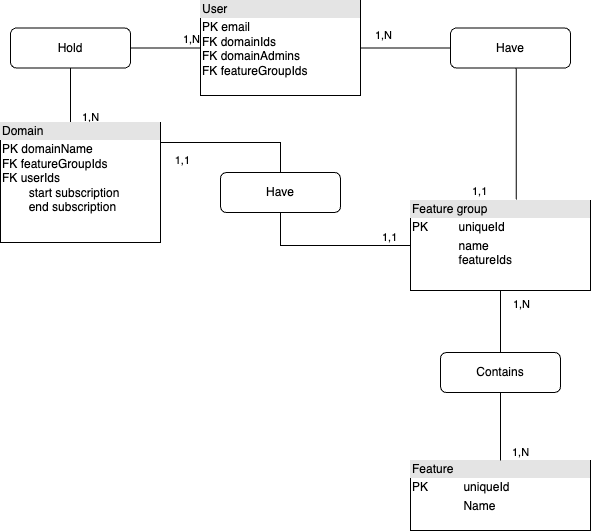
\includegraphics[scale=0.40,center]{schemas/features-mcd-ralph2.png}
      \caption{Modèle de conception de données des domaines clients}
  \end{figure}
  \begin{figure}[h]
      \centering
      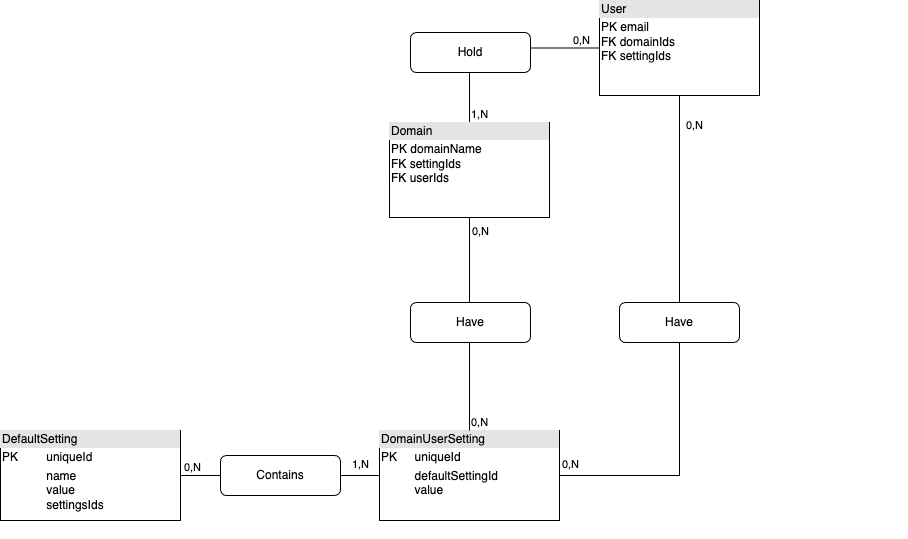
\includegraphics[scale=0.40,center]{schemas/settings-mcd-kingcandy.png}
      \caption{Modèle de conception de données pour la sauvegarde des paramètres clients}
  \end{figure}
  \begin{figure}[h]
      \centering
      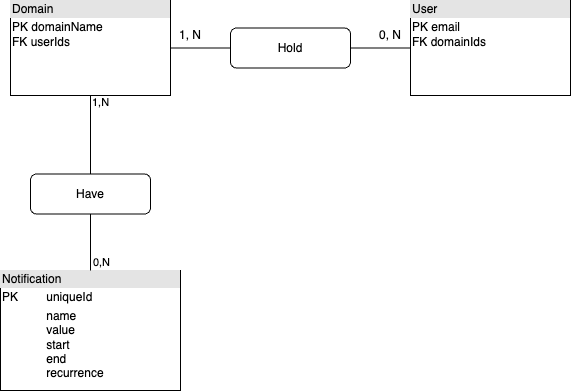
\includegraphics[scale=0.40,center]{schemas/notifications-mcd-calhoun.png}
      \caption{Modèle de conception de données de sauvegarde des paramètres de notifications}
  \end{figure}
  \begin{figure}[h]
      \centering
      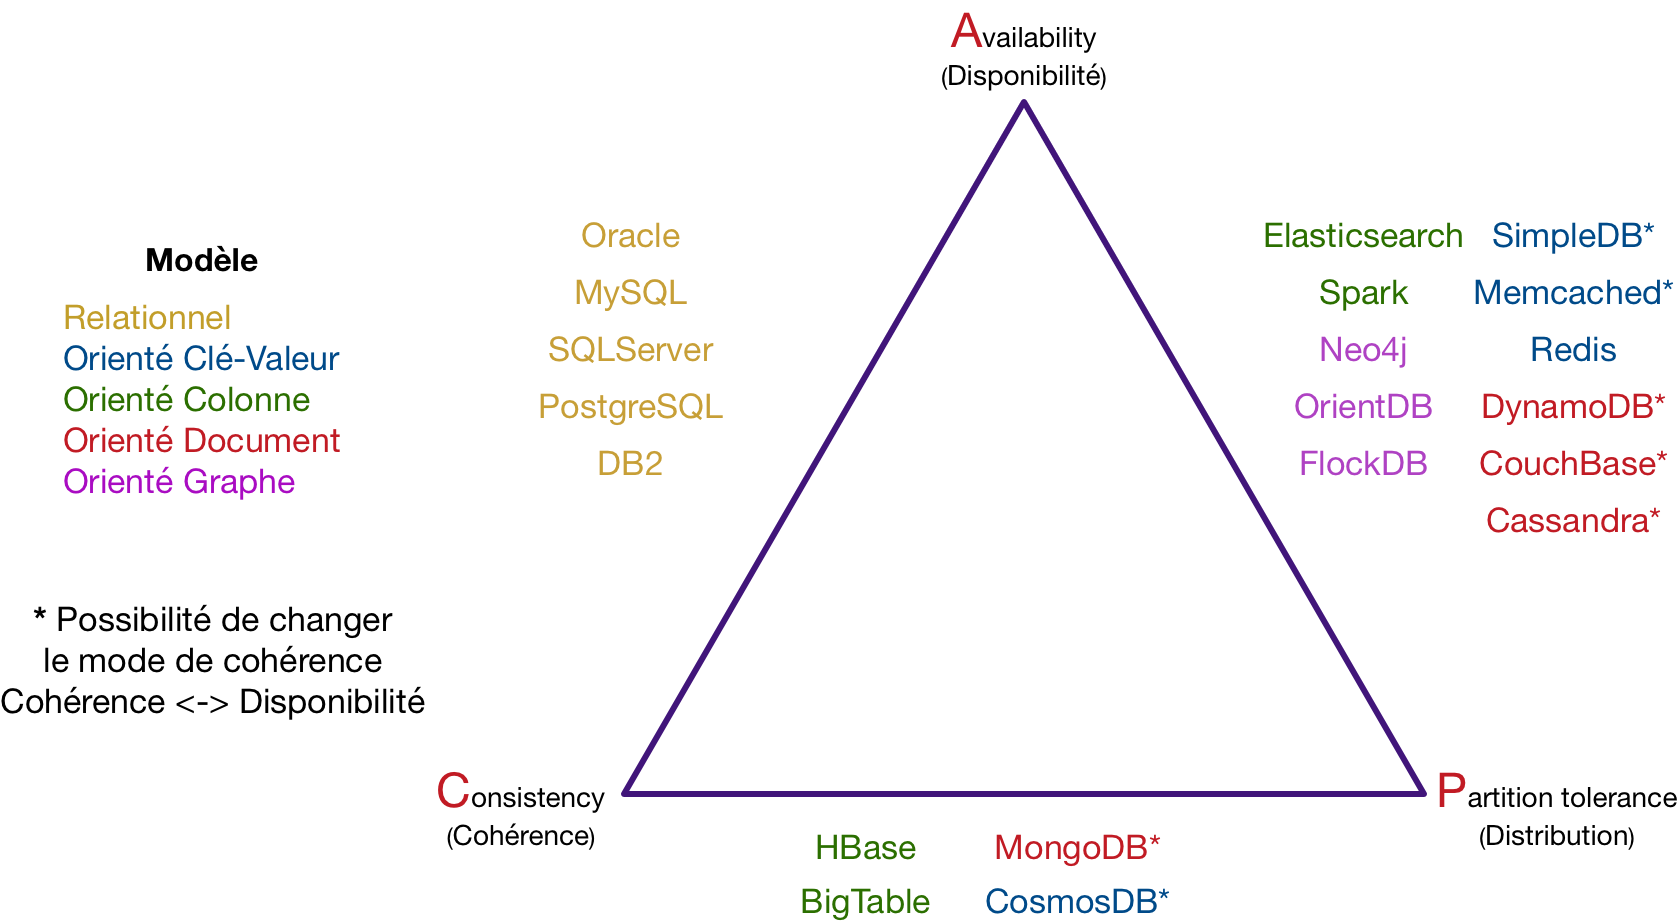
\includegraphics[scale=0.25,center]{schemas/cap-theoreme.png}
      \caption{Théorème CAP}
  \end{figure}
\subsection{Conclusion sur l'activité}

\section{Activité 4 - analyse des besoins métiers pour une solution applicative sur mesure}
\subsection{Compétence et son fondement}
\textbf{Bloc de compétences}: A5 – Développement d’une solution applicative spécifique et métier selon le projet de développement S.I.
\newline
\textbf{Compétence choisie}: A5C1 – Collecter les besoins métiers des utilisateurs en menant des interviews auprès d’eux pour comprendre leurs activités et leurs contraintes métier afin d’étudier les opportunités et la faisabilité technologique d’une solution applicative spécifique ou métier
\subsection{Présentation et réalisation de l'activité}
\subsection{Contexte de réalisation}
\subsection{Conclusion sur l'activité}

\section{Activité 5 - conception d'une architecture applicative évolutive et tolérante aux pannes}
\subsection{Compétence et son fondement}
\textbf{Bloc de compétences}: A5 – Développement d’une solution applicative spécifique et métier selon le projet de développement S.I.
\newline
\textbf{Compétence choisie}: A5C2 – Concevoir une architecture applicative selon la complexité du système d’information existant de type architecture distribuée, ou micro service évolutive et tolérante aux pannes
\subsection{Présentation et réalisation de l'activité}
\subsection{Contexte de réalisation}
  \begin{figure}[h]
      \centering
      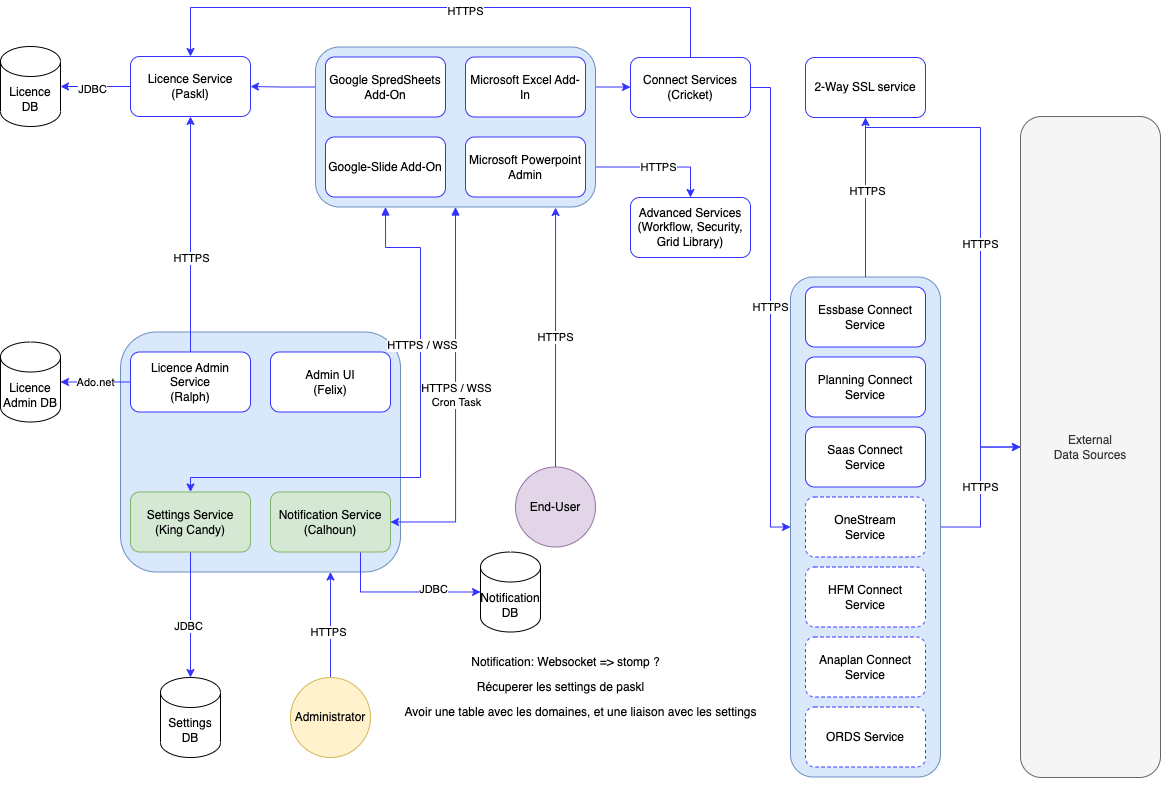
\includegraphics[scale=0.40,center]{schemas/schema-qibates-v2.png}
      \caption{Schéma de la refonte en microservices}
  \end{figure}
\subsection{Conclusion sur l'activité}

\section{Activité 6 - développement d'une application pour répondre aux besoins utilisateurs/directions métiers}
\subsection{Compétence et réalisation et son fondement}
\textbf{Bloc de compétences}: A5 – Développement d’une solution applicative spécifique et métier selon le projet de développement S.I.
\newline
\textbf{Compétence choisie}: A5C3 Développer une application adéquate selon la stratégie applicative de l’environnement en utilisant un langage de programmation approprié dans le respect du cahier des charges établi afin de répondre aux besoins utilisateurs/directions métiers
\subsection{Présentation et réalisation de l'activité}
\subsection{Contexte de réalisation}
\subsection{Conclusion sur l'activité}

\section{Activité 7 - analyse de la qualité de la solution applicative et mise en place d’un plan de correction / d’amélioration}
\subsection{Compétence et son fondement}
\textbf{Bloc de compétences}: A5 – Développement d’une solution applicative spécifique et métier selon le projet de développement S.I.
\newline
\textbf{Compétence choisie}: A5C5 – Effectuer les tests de la solution applicative paramétrée ou développée pour identifier les erreurs et dysfonctionnements et établir les plans de correction/d’amélioration avant sa mise en production
\subsection{Présentation et réalisation de l'activité}
\subsection{Contexte de réalisation}
\subsection{Conclusion sur l'activité}

\section{Activité 8 - mise en place d’une solution d’intégration continue}
\subsection{Compétence et son fondement}
\textbf{Bloc de compétences}: A5 – Développement d’une solution applicative spécifique et métier selon le projet de développement S.I.
\newline
\textbf{Compétence choisie}: A5C6 –Appliquer l’intégration continue dans le cadre du développement d’une application en utilisant un outil d’intégration continue afin de vérifier la conformité de la solution et les besoins utilisateurs
\subsection{Présentation et réalisation de l'activité}
\subsection{Contexte de réalisation}
\subsection{Conclusion sur l'activité}

\section{Activité 9 - validation fonctionnelle et rédaction de la documentation pour les utilisateurs}
\subsection{Compétence et son fondement}
\textbf{Bloc de compétences}: A5 – Développement d’une solution applicative spécifique et métier selon le projet de développement S.I.
\newline
\textbf{Compétence choisie}: A5C7 – Vérifier la conformité entre la solution développée ou paramétrée et les fonctionnalités attendues à partir des retours des directions métiers afin de rédiger la documentation et les référentiels orientés utilisateurs
\subsection{Présentation et réalisation de l'activité}
\subsection{Contexte de réalisation}
\subsection{Conclusion sur l'activité}

\section{Activité 10 - formation des utilisateurs, mise en place d’une enquête de satisfaction ultérieure}
\subsection{Compétence et son fondement}
\textbf{Bloc de compétences}: A5 – Développement d’une solution applicative spécifique et métier selon le projet de développement S.I.
\newline
\textbf{Compétence choisie}: A5C8 - Conduire le changement auprès des métiers lors du déploiement d’une solution applicative ou intégrée en mettant en place une démarche de participation, de communication et de formation pour accompagner les utilisateurs à l’intégration du nouvel outil dans leurs habitudes de travail
\subsection{Présentation et réalisation de l'activité}
\subsection{Contexte de réalisation}
\subsection{Conclusion sur l'activité}

\chapter{Conclusion}

\section{Résumé}
Ce projet m'a permis d'acquérir une expérience précieuse dans le dévelop\-pement de microservices, en utilisant une combinaison de technologies telles que PostgreSQL, Spring Boot et Angular.
La réalisation de ce projet m'a permis de mettre en pratique mes connaissances théoriques acquises au cours de mes études.
J'ai dû faire face à des défis techniques, tels que la modélisation de la base de données et la mise en œuvre des fonctionnalités clés de l'application.
Ce projet m'a également sensibilisé à l'importance de la planification, de la gestion du temps et de la communication efficace dans un contexte professionnel.
J'ai appris à hiérarchiser les tâches, à gérer les priorités et à respecter les délais, tout en maintenant une communication régulière avec mon équipe et en fournissant des mises à jour régulières sur l'avancement du projet.
\newline
\newline
En conclusion, ce projet de gestion des licences utilisateurs chez Quartz-Insight a été une expérience enrichissante qui m'a permis de consolider mes compétences en développement de microservices et en gestion de projet de bout-en-bout pour un logiciel.
Je suis fier d'avoir réussi à réaliser un produit fonctionnel et utile pour les entreprises, tout en respectant les exigences et les contraintes du projet.
Je suis reconnaissant envers l'équipe de Quartz-Insight pour leur soutien et leur expertise tout au long du projet.
\section{Ouverture sur l'avenir}

\subsection{L'entreprise et ses perspectives}
Grâce à son expertise approfondie dans le domaine de la BI et de l'EPM, l’entreprise se distingue par sa capacité à proposer des stratégies de gestion efficaces, des modélisations de données précises et des analyses approfondies pour aider les entreprises à prendre des décisions éclairées.
Son équipe de consultants hautement qualifiés travaille en étroite collaboration avec les clients pour comprendre leurs besoins spécifiques et résoudre leurs problèmes, voir être pro-actifs par rapport à ceux-ci.
\newline
\newline
Les perspectives de Quartz-Insight en tant que PME sont prometteuses.
Avec son approche personnalisée, son agilité et son engagement continu envers l'innovation, l'entreprise est bien positionnée pour étendre sa clientèle et se démarquer sur le marché de la BI et de l'EPM.
La taille réduite de l'entreprise lui permet également de maintenir une culture d'entreprise forte et un haut niveau de service client, ce qui contribue à sa réputation positive.

\subsection{Le service et ses évolutions}
Grâce à la vente de licences en constante augmentation, auprès d’une clientèle de plus en plus variée, la pérennité du service est assurée. Mais de nouvelles contraintes et nouvelles améliorations peuvent être mises en place:
\begin{enumerate}
  \item \textbf{Ajout de nouveaux connecteurs et intégration de nouvelles sources de données}:
    \ En permettant l'intégration de nouvelles sources de données, telles que des bases de données supplémentaires, des services cloud ou des API externes, les utilisateurs auront une plus grande flexibilité dans l'exploration de diverses sources.
  \item \textbf{Amélioration de la supervision}:
    \ En intégrant des fonctionnalités de supervision avancées, telles que des tableaux de bord de surveillance en temps réel, des alertes automatisées en cas d'anomalies ou de dépassement de seuils, et des rapports de performance détaillés, les administrateurs et responsables pourront superviser efficacement les performances et l'utilisation de Qibates.
    \ Cela facilitera la détection précoce des problèmes, l'optimisation des ressources et la prise de décisions basées sur des données précises.
  \item \textbf{Élaboration d'un Plan de Reprise d'Activité (PRA)}:
    \ Pour assurer la continuité des opérations en cas d'incident majeur ou de catastrophe, il est essentiel de développer un PRA solide pour Qibates.
    \ Ce plan devrait inclure des procédures détaillées pour la sauvegarde régulière des données, la restauration du système, la reprise des opérations critiques, la communication avec les parties prenantes, ainsi que des tests réguliers pour s'assurer de l'efficacité du plan.
    \ Un PRA bien élaboré garantira une reprise rapide et efficace des activités en cas d'urgence, minimisant ainsi l'impact sur les utilisateurs et l'entreprise dans son ensemble.
  \item \textbf{Amélioration de la documentation}:
    \ En fournissant une documentation détaillée et des ressources de support, la prise en main de Qibates par les utilisateurs seras facilitée.
\end{enumerate}

\subsection{Les apports professionnels et personnels}
Ce projet réalisé au sein de Quartz-Insight lors de mon alternance a été une expérience professionnelle et personnelle enrichissante.
Sur le plan professionnel, j'ai pu mettre en pratique mes compétences techniques en développement de microservices, en utilisant des technologies telles que PostgreSQL, Spring Boot et Angular.
J'ai renforcé ma compréhension des processus de développement logiciel et des bonnes pratiques. 
Travailler en équipe m'a permis d'améliorer ma communication et ma collaboration.
Sur le plan personnel, j'ai gagné en confiance en moi grâce aux succès obtenus et j'ai développé mon autonomie en prenant des initiatives et en résolvant des problèmes de manière indépendante.
En résumé, ce projet m'a apporté des compétences techniques solides, renforcé ma confiance en moi, développé mon autonomie et élargi mon réseau professionnel, ce qui constituera des atouts précieux pour ma future carrière en tant qu'ingénieur logiciel.

\subsection{Avenir professionnel}
Pour mon avenir professionnel, je suis passionné par l'optimisation des performances en tant qu'ingénieur en logiciel. Je suis attiré par le développ\-ement frontend avec des langages et libraries tels que TypeScript, React ou Svelte, ainsi que le développement backend avec Rust. Mon objectif est de créer des applications web rapides et performantes en réduisant les temps de réponse et en optimisant les requêtes.
J'explore également l'utilisation de Rust compilé en WebAssembly pour exécuter du code hautement performant dans les navigateurs web. Cela me permet de développer des applications web puissantes et réactives, offrant une expérience utilisateur améliorée.
En résumé, mon ambition est de contribuer à des projets stimulants axés sur l'amélioration des performances. Je souhaite devenir un ingénieur en logiciel polyvalent, capable de créer des solutions performantes en utilisant React ou Svelte, TypeScript, Rust et WebAssembly, afin de garantir des expériences utilisateur exceptionnelles et d'optimiser l'efficacité des systèmes.

\end{document}
